\chapter{PredictionIO}\label{c:predictionio}

Apache PredictionIO è un software open source che permettere di sviluppare dei server per il machine learning per qualsiasi task, in particolare è possibile creare degli engines, o modificarne di già esistenti per adattarli alle proprie esigenze, per gestire uno o più algoritmi di machine learning. Le sue funzionalità sono:
\begin{itemize}
\item implementare degli engines ed effetturane il deploy come web service,
\item interrogare un engine con delle query dinamiche e ricevere risposte in real-time,
\item valutare e modificare un engine in modo dinamico,
\item creare un proprio modello di machine learning e implementarlo in un nuovo engine.
\end{itemize}
Da settembre 2020 Apache PreditcionIO è stato messo "nell'attico" da Apache, il che significa che non sarà più supportato e aggiornato da chi l'ha sviluppato, ma è ancora perfettamente funzionante e ho scelto di utilizzarlo perchè credo che le sue funzionalità portino valore nel software development e consentano agli sviluppatori software di integrare algoritmi di machine learning in modo agevole e veloce.

\section{Architettura di PredictionIO}
Apache PredictionIO si integra con applicazioni mobile, web o desktop, le quali possono inviare dei dati all'\textbf{event server}, il quale conserverà i dati, appoggiandosi al database HBase di Apache, i quali saranno poi utilizzati per l'addestramento del modello. L'applicazione potrà mandare dati all'event server in qualsiasi momento, anche dopo il deploy e l'engine di PredictionIO potrà aggiornarsi in modo dinamico effettuando un continuo addestramento che gli permetterà di adattarsi ai dati che gli utenti dell'applicazione continueranno a produrre.

\begin{figure}[!h]
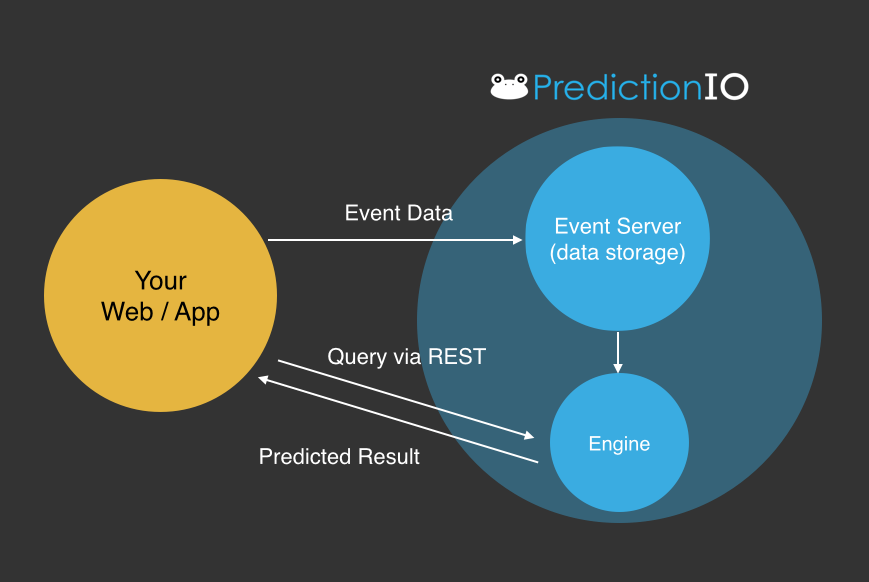
\includegraphics[width=1.0\textwidth]{immagini/app_integration.png}
\caption{Architettura di PredictionIO \cite{sitopredictionio}}
\label{fig:app_integration}
\end{figure}

L'engine o gli engines implementati per l'applicazione si interfacceranno con l'event server per leggere i dati e fare l'addestramento, inoltre potranno ricevere delle richieste tramite query REST dall'app e risponderanno in real-time fornendo la previsione.

\section{Event Server}
L'event server è la componente che memorizza i dati inviati dall'applicazione. Questi dati sono salvati in un database, in particolare viene usato HBase, e verranno mandati al modello nel momento dell'addestramento. I dati vengono salvati con uno stile \textit{event-based}: l'applicazione manda "eventi" che avranno determinate caratteristiche e attributi a seconda del task del modello. Ogni evento ha un "entityType" che rappresenta il tipo di entità che quell'evento rappresenta e può essere personalizzato dallo sviluppatore a seconda dei propri dati (ad esempio "user", "item", "product"...); un "entityId" per identificare l'entità di quell'evento, e altri attributi definiti dallo sviluppatore per descrivere le entità che devono essere rappresentate. Infine gli eventi possono essere di tre tipi:

\begin{itemize}
\item \textbf{"\$set"}: per inserire una nuova entità o modificare gli attributi di una già esistente.
\item \textbf{"\$unset"}: per mantenere un'entità in memoria ma considerarla come se fosse eliminata.
\item \textbf{"\$delete"}: per eliminare un'entità.
\end{itemize}

\newpage

\begin{figure}[!ht]
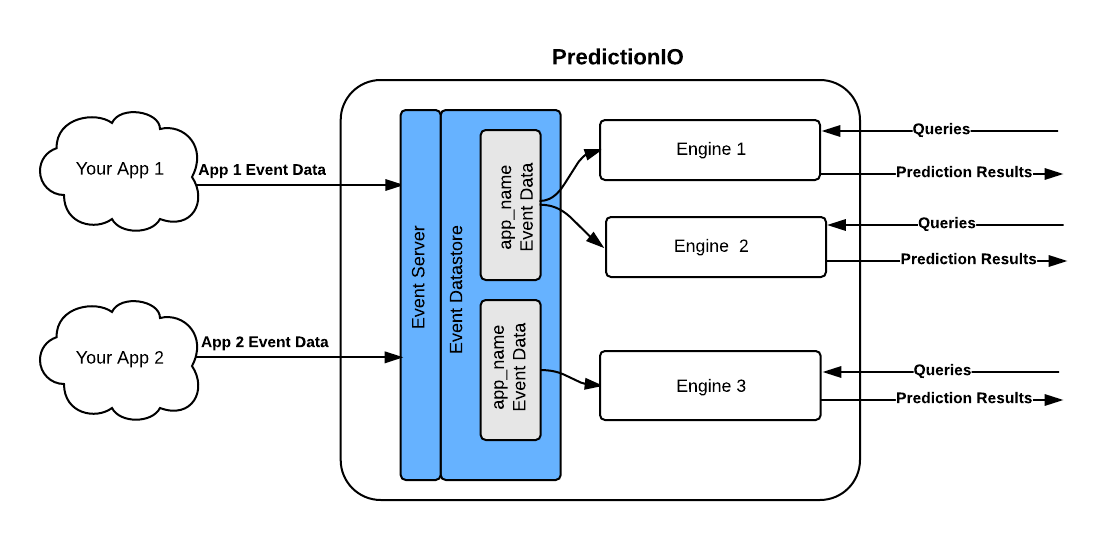
\includegraphics[width=1.0\textwidth]{immagini/eventserver.png}
\caption{Event Server \cite{sitopredictionio}}
\label{fig:eventserver}
\end{figure}

L'event server deve essere attivato anch'esso come servizio web prima di poter ricevere dei dati e prima di mandarli al modello per l'addestramento. Con il comando \verb+pio eventserver+ l'event server viene avviato e sarà disponibile di default all'indirizzo http://localhost:7070.

L'event server può contenere i dati di più engines quindi è necessario specificare a quale modello ogni dato è riferito. Per farlo si creano, con il comando \verb+pio app new myapp+, delle \textit{pio app} relative ad un solo engine, ogni app avrà come identificatore una \textit{access key} che sarà specificata nei dati che vengono mandati all'event server. In questo modo quando sarà il momento di addestrare un modello l'event server fornirà i dati solo relativi all'access key di quell'engine.

\section{Engines come servizi web}
Un engine è un'identità logica che rappresenta un algoritmo di machine learning per un determinato task, può interagire con una sola applicazione ed è specifico per un determinato task, mentre un'applicazione può interagire con più engines. Gli engine possono essere di diverso tipo:
\begin{itemize}
\item raccomandazione: per task relativi a "raccomandare" prodotti sulla base di preferenze e gusti di un utente,
\item classificazione: per task relativi a classificare un determinato target, si basa sui principali algoritmi di classificazione,
\item regressione: per task per valutare un target con un valore continuo, quindi si basa sugli algoritmi di regressione.
\end{itemize}

Le funzioni di un engine quindi sono quelle di leggere i dati dall'event server per l'addestramento del modello che l'engine rappresenta, dopodichè viene fatto il deploy come servizio web e infine deve rispondere alle richieste ricevute dall'applicazione facendo predizioni.

\subsection{DASE}
Un engine è strutturato con un'architettura che prende il nome di \textbf{DASE}, acronimo di \textbf{D}ata Source and Preparator, \textbf{A}lgorithm, \textbf{S}erving e \textbf{E}valuation Metrics. 
\begin{itemize}
\item \textbf{Data Source e Preparator}: la componente di data source prende i dati in input e li trasforma nel formato desiderato dal modello di machine learning che viene utlizzato; mentre la componente di data preparator prende i dati processati dal data source e li manda in input all'algoritmo per l'addestramento.
\item \textbf{Algorithm}: la componente algorithm include l'algoritmo di machine learning vero e proprio, con il settaggio dei parametri e determina come il modello è costruito. La componente algorithm si basa sulla piattaforma Apache Spark, in particolare sulla libreria Spark's MLLib (machine learning library), che gestirà tutta la parte di addestramento dell'algoritmo scelto.
\item \textbf{Serving}: la componente di serving ha il compito di ricevere in input le richieste dell'applicazione, mandarle al modello e rispondere con il risultato predetto.
\item \textbf{Evaluation Metrics}: la componente di evaluation valuta le performance del modello e ne dà un risultato numerico, può essere usata quindi per fare comparazioni tra diversi algoritmi.
\end{itemize}

\begin{figure}[!h]
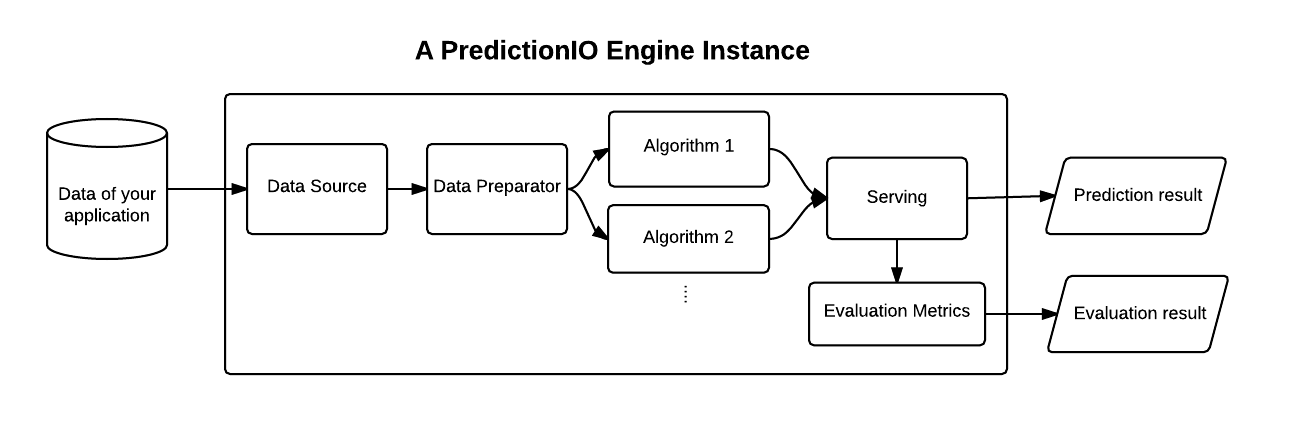
\includegraphics[width=1.0\textwidth]{immagini/dase.png}
\caption{Architettura DASE \cite{sitopredictionio}}
\label{fig:dase}
\end{figure}

\subsection{Addestramento e deploy}
Un engine quindi consiste nelle varie componenti DASE che sono implementate in un proggetto nel linguaggio Scala, un linguaggio orientato agli oggetti la cui compilazione produce bytecode java eseguibile su una Java Virtual Machine. Sono disponibili molti engine template per i vari tipi disponibili, in modo che uno sviluppatore possa partire da uno di questi template già pronti, con le vari componenti DASE già implementate e andare a modificare le componenti solo per adattarle al proprio task specifico, altrimenti è anche possibile svilupparlo da zero.

Una volta implementato un engine, è necessario eseguire una serie di operazioni per renderlo operativo:
\begin{itemize}
\item \textbf{build del progetto}: con il comando \verb+pio build+ viene eseguito il build del progetto,
\item \textbf{training}: con il comando \verb+pio train+ l'engine legge i dati relativi al suo modello dall'event server ed esegure l'addestramento dell'algoritmo,
\item \textbf{deploy come servizio web}: dopo aver correttamente addestrato il modello è possibile eseguirne il deploy con il comando \\ \verb+pio deploy --port 8000+, in questo modo il modello sarà disponibile come servizio web alla porta specificata nel comando, in questo caso alla porta 8000.
\end{itemize}

\begin{figure}[!h]
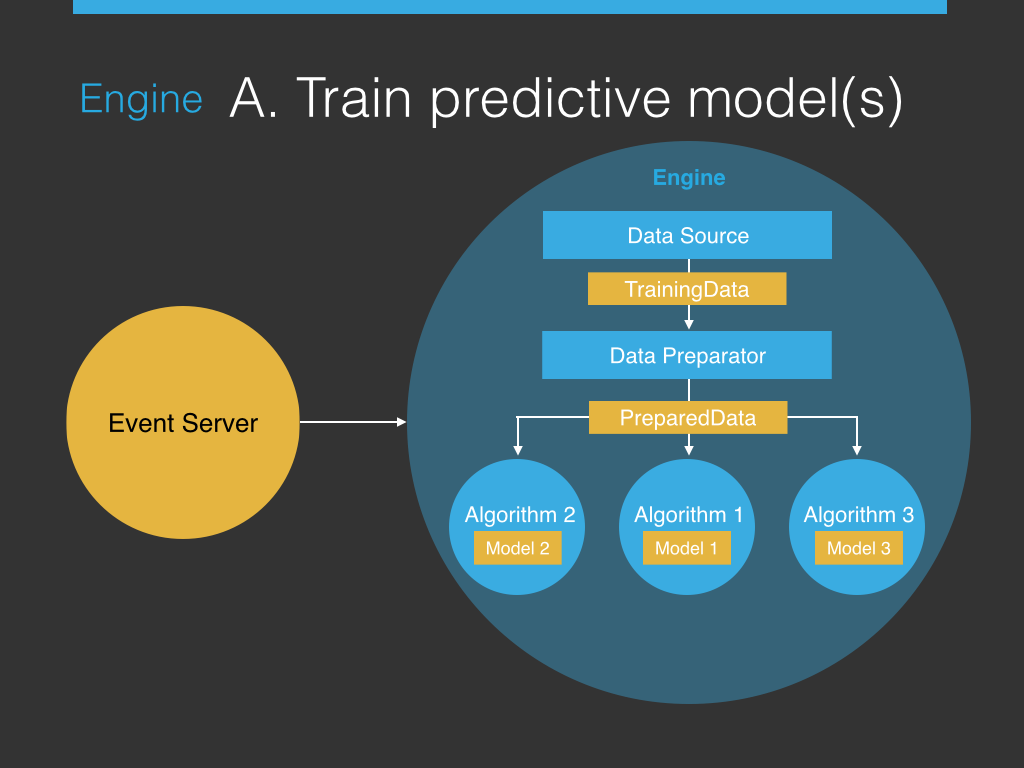
\includegraphics[width=0.8\textwidth]{immagini/training.png}
\caption{Addestramento \cite{sitopredictionio}}
\label{fig:training}
\end{figure}

Dopo aver eseguito questi passaggi è possibile fare richieste al modello con query REST all'indirizzo http://localhost:8000 (nel caso l'engine sia operativo sulla macchina locale). L'applicazione che dovrà interagire con il modello potrà sfruttare le API's di PredictionIO disponibili per i principali linguaggi di programmazione(Java, Python, Ruby, PHP...).

\begin{figure}[!h]
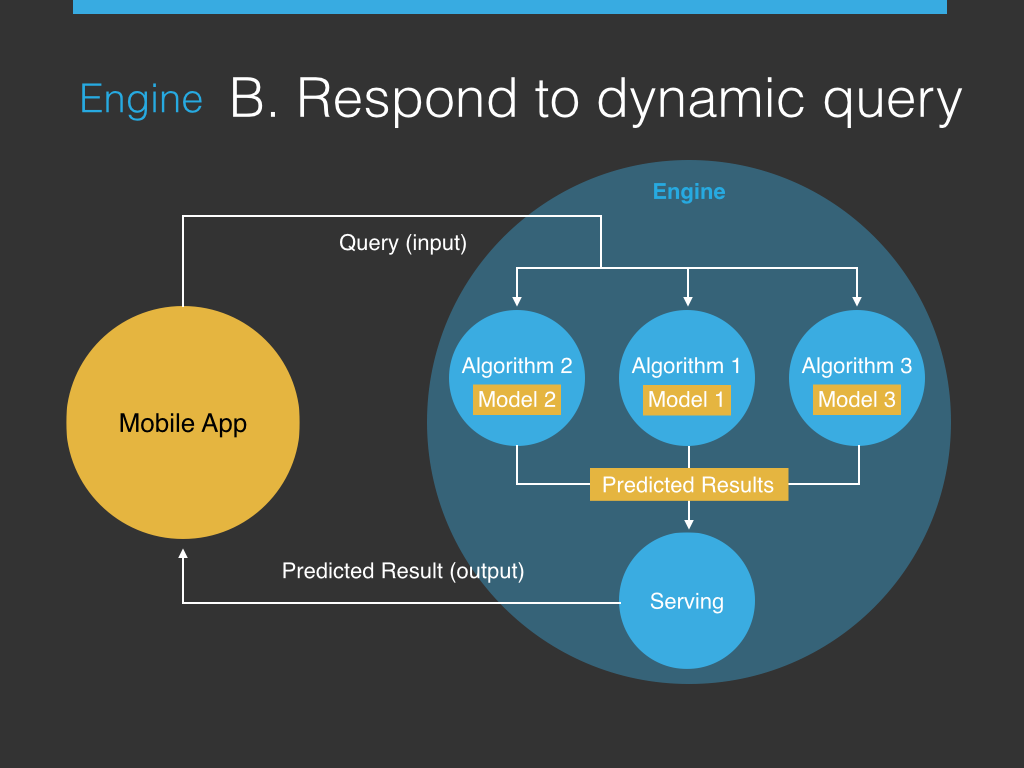
\includegraphics[width=0.8\textwidth]{immagini/deploy.png}
\caption{Interazione app-engine \cite{sitopredictionio}}
\label{fig:deploy}
\end{figure}

\newpage

\section{Installazione con Docker}
Il software PredictionIO può essere installato in modo nativo su una qualsiasi macchina UNIX. In questo caso però è necessario gestire manualmente tutte le numerose dipendenze e potrebbero sorgere problemi di compatibilità. Per lo svolgimento di questo elaborato è stato quindi scelto di installare il software utilizzando Docker.

\subsection{Docker}
Docker consente di automatizzare il deploy di software all'interno di \textbf{container} software, aggiungendo un livello di astrazione grazie alla virtualizzazione del sistema operativo Linux. Lo scopo di Docker quindi è quello di fornire dei "package" che contengono un software installato con tutte le sue dipendenze in modo da essere già pronto per il deploy, e quindi facilmente utilizzabile. A differenza delle classiche macchine virtuali Docker fornisce container più leggeri e più isolati, che possono essere installati a prescindere dalla macchina host che li ospiterà garantendo forte granularità e portabilità.

\subsection{PreditionIO con Docker}
PredictionIO fornisce piena compatibilità con Docker ed è facilmente installabile utilizzando il container già disponibile. Una volta scaricato il software open source di PredictionIO si può installare l'immagine Docker facilmente con il comando \verb+docker build -t predictionio/pio pio+, dove il software di PredictionIO è nella directory chiamata \verb+predictionio+ (l'unico requisito è avere Docker installato e funzionante sulla propria macchina). Dopodiché dalla sottocartella \verb+predictionio/docker+ è possibile avviare PredictionIO e utilizzare i comandi già visti prima per creare engine ed eseguire i vari passaggi, con l'unica differenza di usare il comando \verb+pio-docker+ al posto di \verb+pio+.